\subsection{Computer simulations}

We have built a virtual environment including various racing circuits in Unreal Engine for testing the reactive planning and control algorithm.
%
% Our planner and controller is simple yet can safely complete a variety of tracks.
%
Some of these tracks are provided in Figure~\ref{fig:simulation_tracks}.
%
The tracks in the left column are similar to the tracks on which F1Tenth competitions \cite{f1tenth} were conducted.
Other tracks include a triangular track, and a straight track with static obstacles.
%
We have also tested the simulation on some polygonal tracks for which we will provide formal analysis in the subsequent sections.
%
Videos of these simulations are available on the web.\footnote{\url{https://tinyurl.com/ry5xhza}}
%
In total, of the nine different laps that we have tested, our algorithm was able to successfully able to complete a lap while not colliding with any of the race track boundaries or obstacles.

\begin{figure}[!t]
\centering
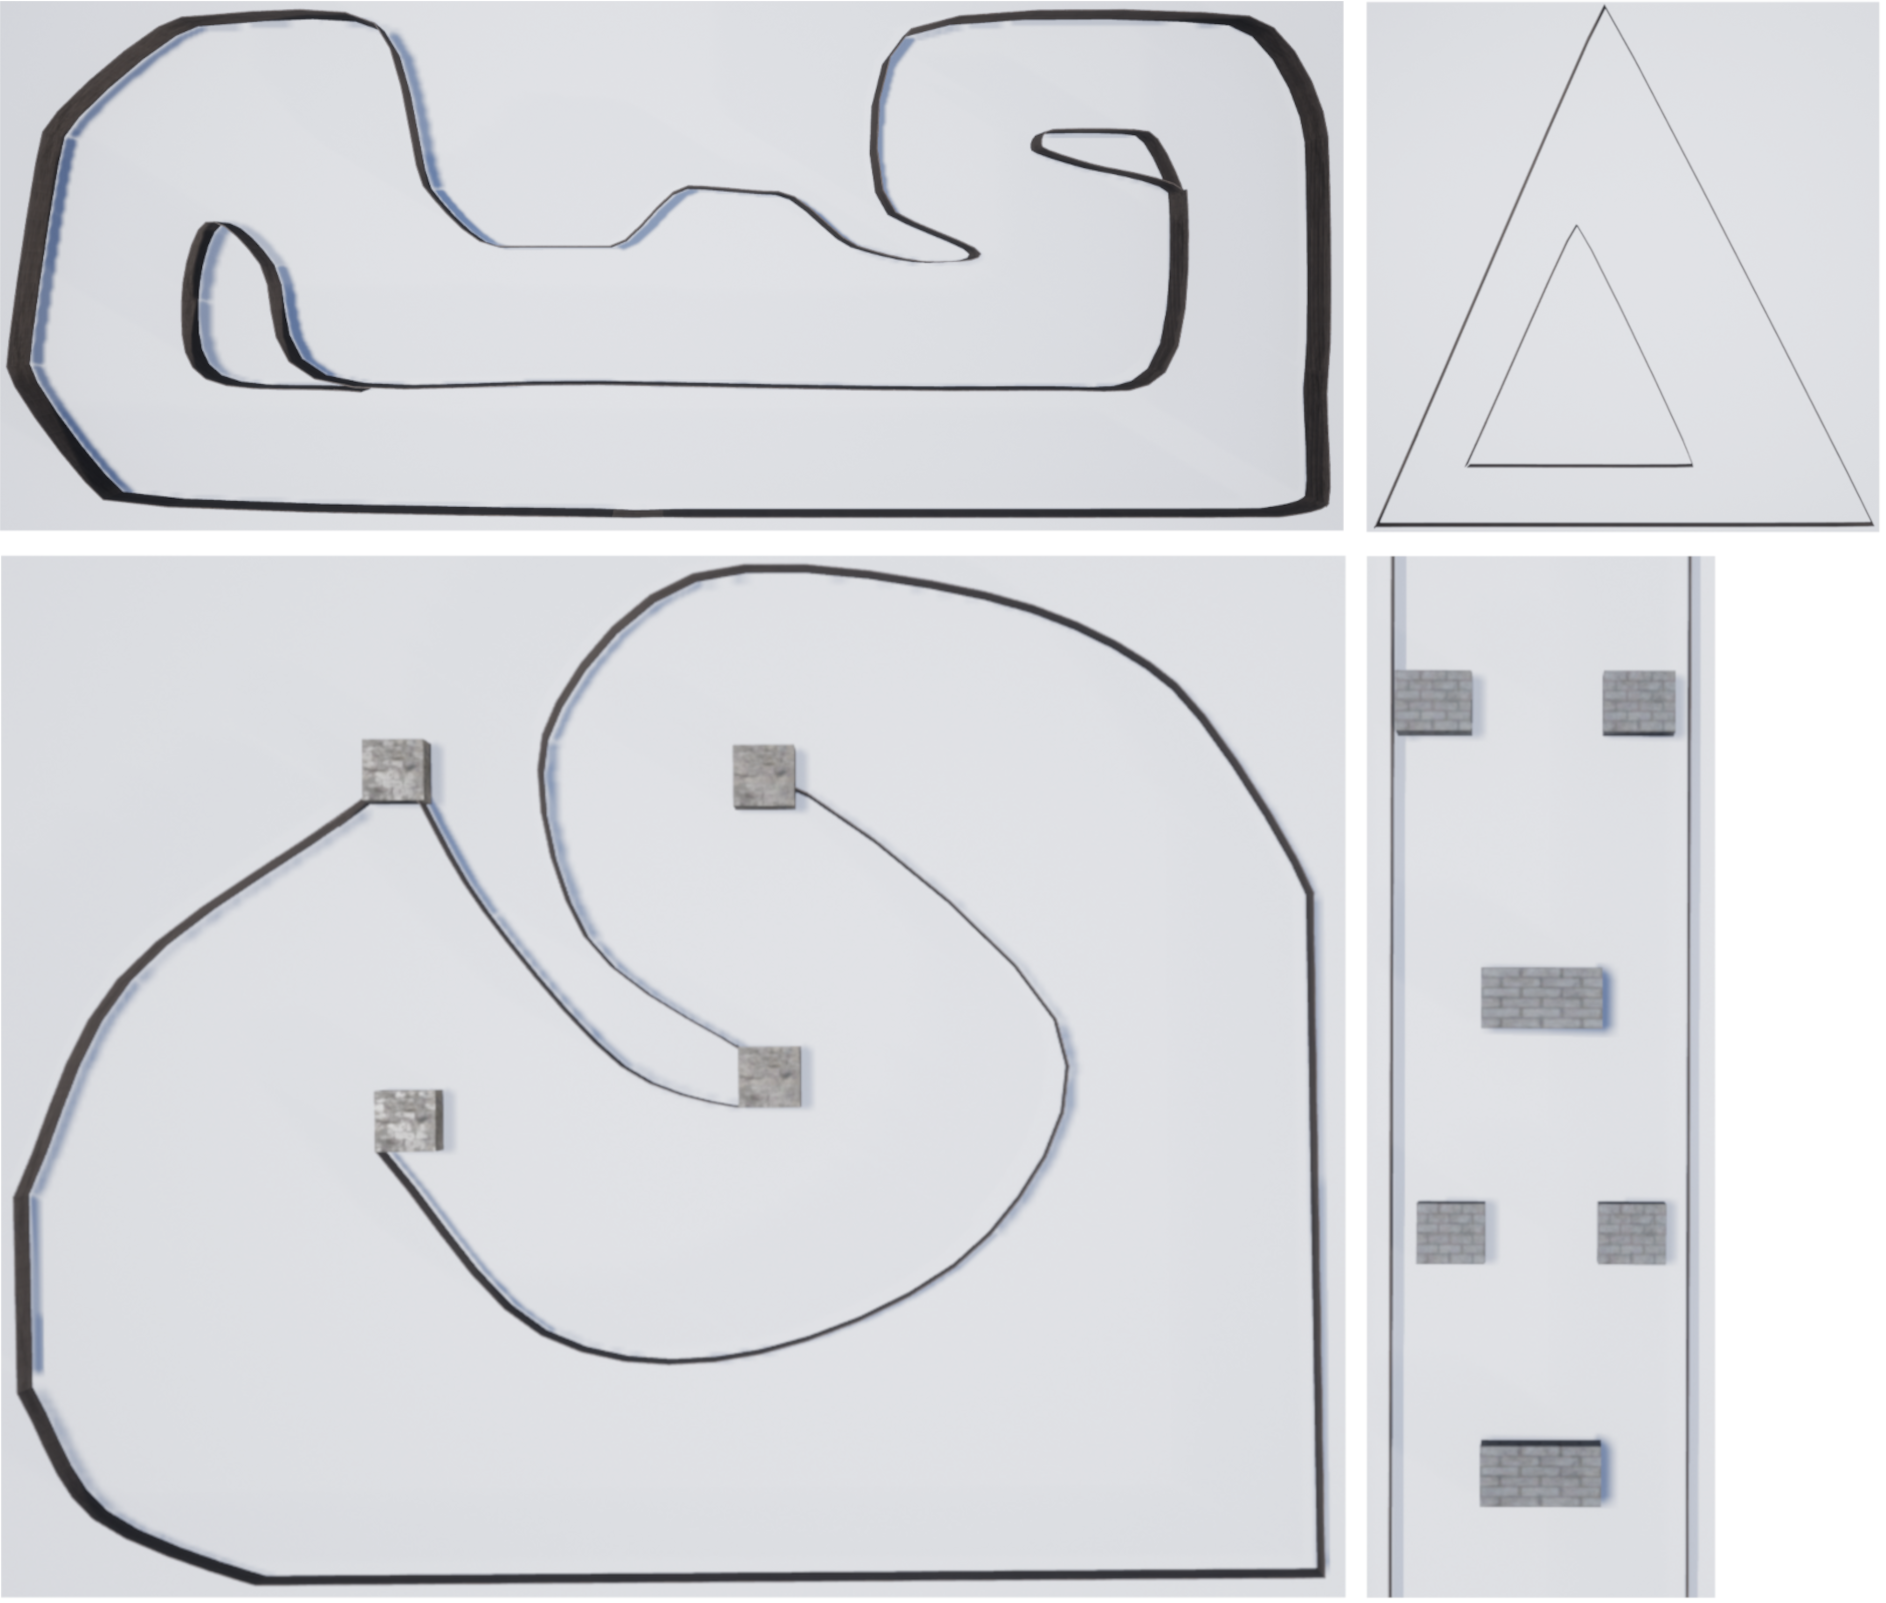
\includegraphics[width=0.8\columnwidth]{Figures/sim-tracks.png}
\caption{Racing tracks for the simulations.}
\label{fig:simulation_tracks}
\end{figure}

The vehicle used in the simulations is the vehicle from Unreal Engine 4.21's `Vehicle Advanced' template project.
The default tire friction constants are increased to avoid wheel slippage.
We have implemented a model of Hokuyo UST-10LX LiDAR in Unreal Engine.
The measurements are taken using Unreal Engine's line tracing.
We do not model measurement errors and uncertainty.


